\documentclass[10pt]{beamer}

% --- Layout ---
\usetheme{Madrid}
\usecolortheme{beaver}
\setbeamersize{text margin left=1.5cm, text margin right=1.5cm}
\usecolortheme{dolphin}
\setbeamertemplate{navigation symbols}{}

% --- Sprache / Mathe ---
\usepackage[utf8]{inputenc}
\usepackage{amsmath, amssymb}

% --- schöneres Layout ---
\setlength{\parskip}{0.4em}



\title{Rechnen mit ganzen Zahlen}
\author{Alisa Mirena}
\date{28.04.2026}

\begin{document}


\frame{\titlepage}

\begin{frame}
\frametitle{Inhaltsverzeichnis}

1. Addition und Subtraktion

2. Multiplikation

3. Euklidischer Algorithmus

\end{frame}

\section{Einleitung}

\begin{frame}
\frametitle{1. Addition und Subtraktion}
Der Algorithmus hat Laufzeit $O(l)$, wobei $l$ die maximale Anzahl an Stellen der beteiligten Zahlen ist. $O(l)$ wächst proportional, d.h. wenn die Zahlen mit denen man rechnet doppelt so lang werden, dann wird auch die Rechnung doppelt so lang.
\end{frame}

\section{Hauptteil}

\begin{frame}
\frametitle{Proposition 1.1 }

Für zwei ganze Zahlen $x$ und $y$ können die Summe $x+y$ und die Differenz $x-y$ in Laufzeit $O(l)$ berechnet werden, wobei
\[
l = 1 + \lfloor \log_2(\max\{|x|, |y|, 1\}) \rfloor.
\]


\end{frame}


\begin{frame}
\frametitle{2.Multiplikation}
    Für die Multiplikation und Division gilt die Laufzeit $O(l^2)$, auch quadratische Laufzeit genannt. 
Der russiche Mathematiker Karatsuba fand im Jahr 1960 als Erster eine Möglichkeit, um Multiplikation noch schneller durchzuführen. Seine Idee war es, die l-stelligen zu multiplizierenden Zahlen x und y in zwei $l/2$-stellige Zahlen zu zerlegen. 
\end{frame}

\begin{frame}
    Damit werden x und y wie folgt dargestellt:

    
\boldsymbol{$x = x'B+x''$}    und    $y=y'B+y''$.
B Ist hierbei die Potenz der Basis.Um das geamte Produkt xy zuerhalten, reicht es die einzelnen Prdukte [$p:= x'y'$], [$q:= x''y''$] und [$r:= (x'+x'') (y'+y'')$] zu berechnen.
\vspace{0.2cm}

 \equation $x\times y = (x'y')B^2+(x'y''+x''y')B+x''y''=pB^2+(r-p-q)B+q$. (2.1)
\end{frame}

\begin{frame}{Beispiel}
Sei $x= 1234$ und $y=5678$.

$x'= 12$ und $x''= 34$; \space $y'=56$ und $y''=78$

$p:= 12\times 56$

$q:= 34\times78$

$r:= (12+34)\times(56+78).$$
\vspace{0.3cm}

 \noindent $x\times y= (12\times56)\times100^2+(12\times78+34\times56)\times100+34\times78= (12\times56)\times100^2+((12+34)\times(56+78)-12\times56-34\times78)\times100+34\times78= 7006654= 1234\times5678$
\vspace{1cm}

 \noindent Das zeigt, dass wir nur 3 einzelne Multiplikationen(r,p,q) durchführen müssen, um das Ergebnis berechnen zu können.
    
\end{frame}

\begin{frame}{Beweis von 2.1}


Erinnerung: $x \times y = (x'y')B^2+(x'y''+x''y')B+x''y''=pB^2+(r-p-q)B+q$. (2.1)


\vspace{0.8cm}
  $x\times y= (x'B+x'')\times(y'B+y'')= x'y'+x'y''B+x''y'B+x''y''= (x'y')B^2+(x'y''+x''y')B+x''y''= pB^2*(r-p-q)B+q$
    
\end{frame}

\begin{frame}{Karatsuba Algorithmus 2.2}

\KwIn{$x, y \in \mathbb{N}$ in Binärdarstellung}
\KwOut{$x \cdot y$ in Binärdarstellung}

\If{$x < 8 \;\text{und}\; y < 8$}{
    \Return $x \cdot y$
}
\Else{

$l \leftarrow 1 + \lfloor \log_2(\max\{x,y\}) \rfloor$\;

$k \leftarrow \lfloor l/2 \rfloor$\;

$B \leftarrow 2^k$\;

$x' \leftarrow \lfloor x/B \rfloor,\quad x'' \leftarrow x \bmod B$\;

$y' \leftarrow \lfloor y/B \rfloor,\quad y'' \leftarrow y \bmod B$\;

$p \leftarrow x' \cdot y'$\; \text{(rekursiv)}

$q \leftarrow x'' \cdot y''$\; \text{(rekursiv)}

$r \leftarrow (x' + x'')(y' + y'')$\; \text{(rekursiv)}

\Return $pB^2 + (r - p - q)B + q$\;

}

\end{frame}


\begin{frame}
    a) Falls $x, y < 8$, dann wird die einfache Multiplikation genutzt.


b) Falls $x, y > 8$, dann wird Karatsubas Algorithmus benutzt.


\vspace{0.5cm}

(Falls x und y nach der Teilung immernoch groß sind, wird der Algorithmus wieder verwendet, bis die Zahlen klein genug sind)

\end{frame}


\begin{frame}{Satz 2.3}

Die Multiplikation zweier in Binärdarstellung gegebener natürlicher Zahlen $x$ und $y$ ist nach der Schulmathematik in Laufzeit $O(l^2)$ möglich. Nach dem Karatsuba-Algorithmus geht dies deutlich schneller. Demnach gilt die Laufzeit $O\left(l^{\log_2 3}\right)$. Wobei weiterhin gilt:
\[
l = 1 + \lfloor \log_2(\max\{x, y, 1\}) \rfloor.
\]
    
\end{frame}

\begin{frame}{Beispiel}

$l = 1 + \lfloor \log_2(\max\{1234, 5678, 1\}) \rfloor = 14$

 $O(l^2)=14^2= 196$ (Rechenschritte)
 
 $O\left(l^{\log_2 3}\right)= 14^1,585= 65,65$

    
\end{frame}

\begin{frame}{Beweis von Satz 2.3}
    z.z.: $T(l) = O\left(l^{\log_2 3}\right)$

\vspace{0.2cm}
$T(l)$:= Laufzeit in Abhängigkeit von Bitlänge $l$. 


\vspace{0.3cm}
\noindent Fall 1.:  $ l \leq 3,: T(l) \leq c$

\vspace{0.3cm}
\noindent Fall 2.: $l \geq 4: T(l) \leq cl+ 3T (\lceil \frac{l}{2} \rceil +1) $

\vspace{0.7cm}

\end{frame}  

\begin{frame}{Induktion}

Setze $ l:= 2^m +2$

\vspace{0.4cm}

\noindent I.B.: $T( 2^m +2) \leq c (4 \times 3^m -2\times 2^m -1)$ für alle $ m \in \mathbf{N_0} $.

\vspace{0.3cm}

\noindent I.A.: $m=0$.

$l= 2^0 +2= 3$.   Nach Fall 1 gilt: $T(3) \leq c$

\vspace{0.3cm}
\noindent I.V.: Ang. $T(2^{m-1} +2) \leq c ( 4\times 3^{m-1} - 2 \times 2^{m-1} -1)$.

    
\end{frame}

    
\begin{frame}

\noindent I.S.: von $(m-1)$ nach $m$.

$T( 2^m +2) \leq c (2^m +2) +3T(\left\lceil \frac{2m+2}{2} \right\rceil +1)$

\vspace{0.2cm}
Da $\frac{2m+2}{2}  +1$ = $2^{m-1}+1$, können wir vereinfachen zu: 

\vspace{0.15cm}
$T( 2^m +2) \leq c (2^m +2) +3T ( 2^{m-1} +2)$ 

\vspace{0.15cm}
(nach I.V.) $\Leftrightarrow $ $T( 2^m +2) \leq+3( c ( 4 \times 3^{m-1} -2 \times 2^{m-1} -1))$

\vspace{0.15cm}
$\Leftrightarrow$ $T(2^m +2) \leq c (2^m +2) + c \times 12 \times 3^{m-1} - c\times 6 \times 2^{m-1} - c \times 3 $

\vspace{0.15cm}
$\Leftrightarrow$  $T(2^m +2) \leq (2^m +2 +12 \times 3^{m-1} - 6 \times 2^{m-1} -3)$

\vspace{0.15cm}

$\Leftrightarrow$ $ T(2^m +2) \leq c( 2^m + 4 \times 3^m -3 \times 2^m -1)$

$\Leftrightarrow $ $T(2^m +2) \leq c (4 \times 3^m -2 \times 2^m -1) $


\vspace{0.4cm}
\noindent Schlussfolgerung: Setze $ m:= \log_2 l $.


\noindent Dann erhalten wir: $T(l) \leq c \times 3^m = c \times 3^{\log_2 l} = c \times l^{\log_2 3} $.

    
\end{frame}


\begin{frame}{3. Euklidischer Algorithmus}

Der Euklidische Algorithmus, beschrieben von Euklid um 300 v.Chr. in Buch VII seiner Elemente, erlaubt das effiziente Brechnen des größten gemeinsamen Teilers zweier Zahlen, und damit das Kürzen von Brüchen.
    
\end{frame}

\begin{frame}{Definition 3.1}
    Seien a,b\in \mathbf{N}. 

\noindent ggT(a,b) ist der größte geinsame Teiler von a und b; d.h. die größte natürliche Zahl, die sowohl a als auch b ganzzahlig teilt. 

Es gelten folgende Eigenschaften:

1) Gilt ggT(a,b)=1, so heißen a und b teilerfremd

2) ggT(a,0):= ggT(0,a):= a  \forall a \in \mathbf{N}.
\end{frame}

\begin{frame}{Definition 3.2}
 KgV(a,b) ist das kleinste gemeinsame Vielfache von a und b; d.h. die kleinste natürliche Zahl, von der sowohl a als auch b Teiler sind.
    
\end{frame}

\begin{frame}{Lemma 3.3}

Es gilt: 

\vspace{0.3cm}
a) $a\times b = ggT(a,b) \times kgV(a,b)$


\noindent b) ggT(a,b)= ggT(a mod b, b)

\end{frame}

\begin{frame}{Beispiel}

Sei a= 10 und b= 8

ggT(a,b)= 2

kgV(a,b)= 40

\vspace{0,5cm}

a) $a \times b= 10 \times 8= 40= 2\times 40 = ggT(a,b) \times kgV(a,b)$

b) $2= ggT(10,8) = ggT (10 \ mod \ 8,8) = ggT(2,8)$
    
\end{frame}

\begin{frame}{Bewies von Lemma 3.3}

a) Teil 1. 
 z.z.:  $a\times b = ggT(a,b) \times kgV(a,b)$ = $\frac{ab}{\text{ggT}(a,b)}$

\vspace{0.5cm}
Sei $\frac{ab}{\text{ggT}(a,b)} := x$

\vspace{0.3cm}
$\frac{ab}{x}$ = $a \left(\frac{b}{x}\right) = $b \left(\frac{a}{x}\right)$

\vspace{0.4cm}
\noindent Da x= ggT(a,b) ist, muss x ein ganzzahliger Teil von b (bzw. a) sein, weshalb auch $\frac{b}{x}$ ganzzahlig ist.
Folglich: $\frac{ab}{x}$ ist ein Vielfaches von a und b.

\noindent Da $\frac{ab}{x}$ ein gemeinsames Vielfaches von a und b ist, muss es größer oder gleich dem kleinsten gemeinsamen Vielfachen sein.

\vspace{0.2cm}
Es folgt: $\frac{ab}{\text{ggT}(a,b)}$ \ge kgV(a,b)

    
\end{frame}

\begin{frame}

Teil 2: 

z.z. $\frac{ab}{\text{kgV}(a,b)}$   \le ggT(a,b)
\vspace{0.2cm}

\noindent Da kgV(a,b) ein Vielfaches von a ist, so exist. ein m, s.d. gilt: $kgV(a,b) = a \times m.$ 

\vspace{=0.2cm}
$\frac{ab}{\text{kgV}(a,b)}$  = $\frac{ab}{am}$ = $\frac{b}{m}$
\vspace{0.3cm}


\noindent Damit ist $\frac{ab}{\text{kgV}(a,b)}$ ein Teiler von b. (a ist analog)

\noindent Da $\frac{ab}{\text{kgV}(a,b)}$ ein gemeinsamer Teiler von a und b ist, muss $\frac{ab}{\text{kgV}(a,b)}$ kleiner oder gleich dem $ggT(a,b)$ sein.
\end{frame}

\begin{frame}
b) 
z.z. ggT(a,b)= ggT(a mod b,b)

\vspace{0.2cm}
$a= b\times q + r$  \iff   $r= a - b\times q$

\noindent Sei d ein Teiler von a und b. Dann gilt: $d | a \iff d | bq+r \iff d | a- bq \iff d | r$

\vspace{0.3cm}
\noindent Damit folgt: $ggT(a,b)= ggT(r,b) = ggT(a \ mod \  b, b)$

\end{frame}


\begin{frame}{Euklidischer Algorithmus 3.4}



Eingabe: $a,b \in \mathbb{N}$ \\
Ausgabe: $\operatorname{ggT}(a,b)$

\begin{align*}
\textbf{while } & a > 0 \text{ und } b > 0 \text{ do} \\
\textbf{if } & a < b \text{ then } b \leftarrow b \bmod a \\
\textbf{else } & a \leftarrow a \bmod b \\
\textbf{output } & \max\{a,b\}
\end{align*}
    
\end{frame}

\begin{frame}{Beispiel}

$a= 48$, $b= 18$
\vspace{0.1cm}


$ggT(48,18)= ggT( 48 \ mod \ 18, 18)= ggT(12,18)= ggT(12,6)=$


\indent $ggT(0,6)= 6 $
    
\end{frame}

\begin{frame}{Euklidischer Algorithmus im Programm}

\begin{figure}
    \centering
    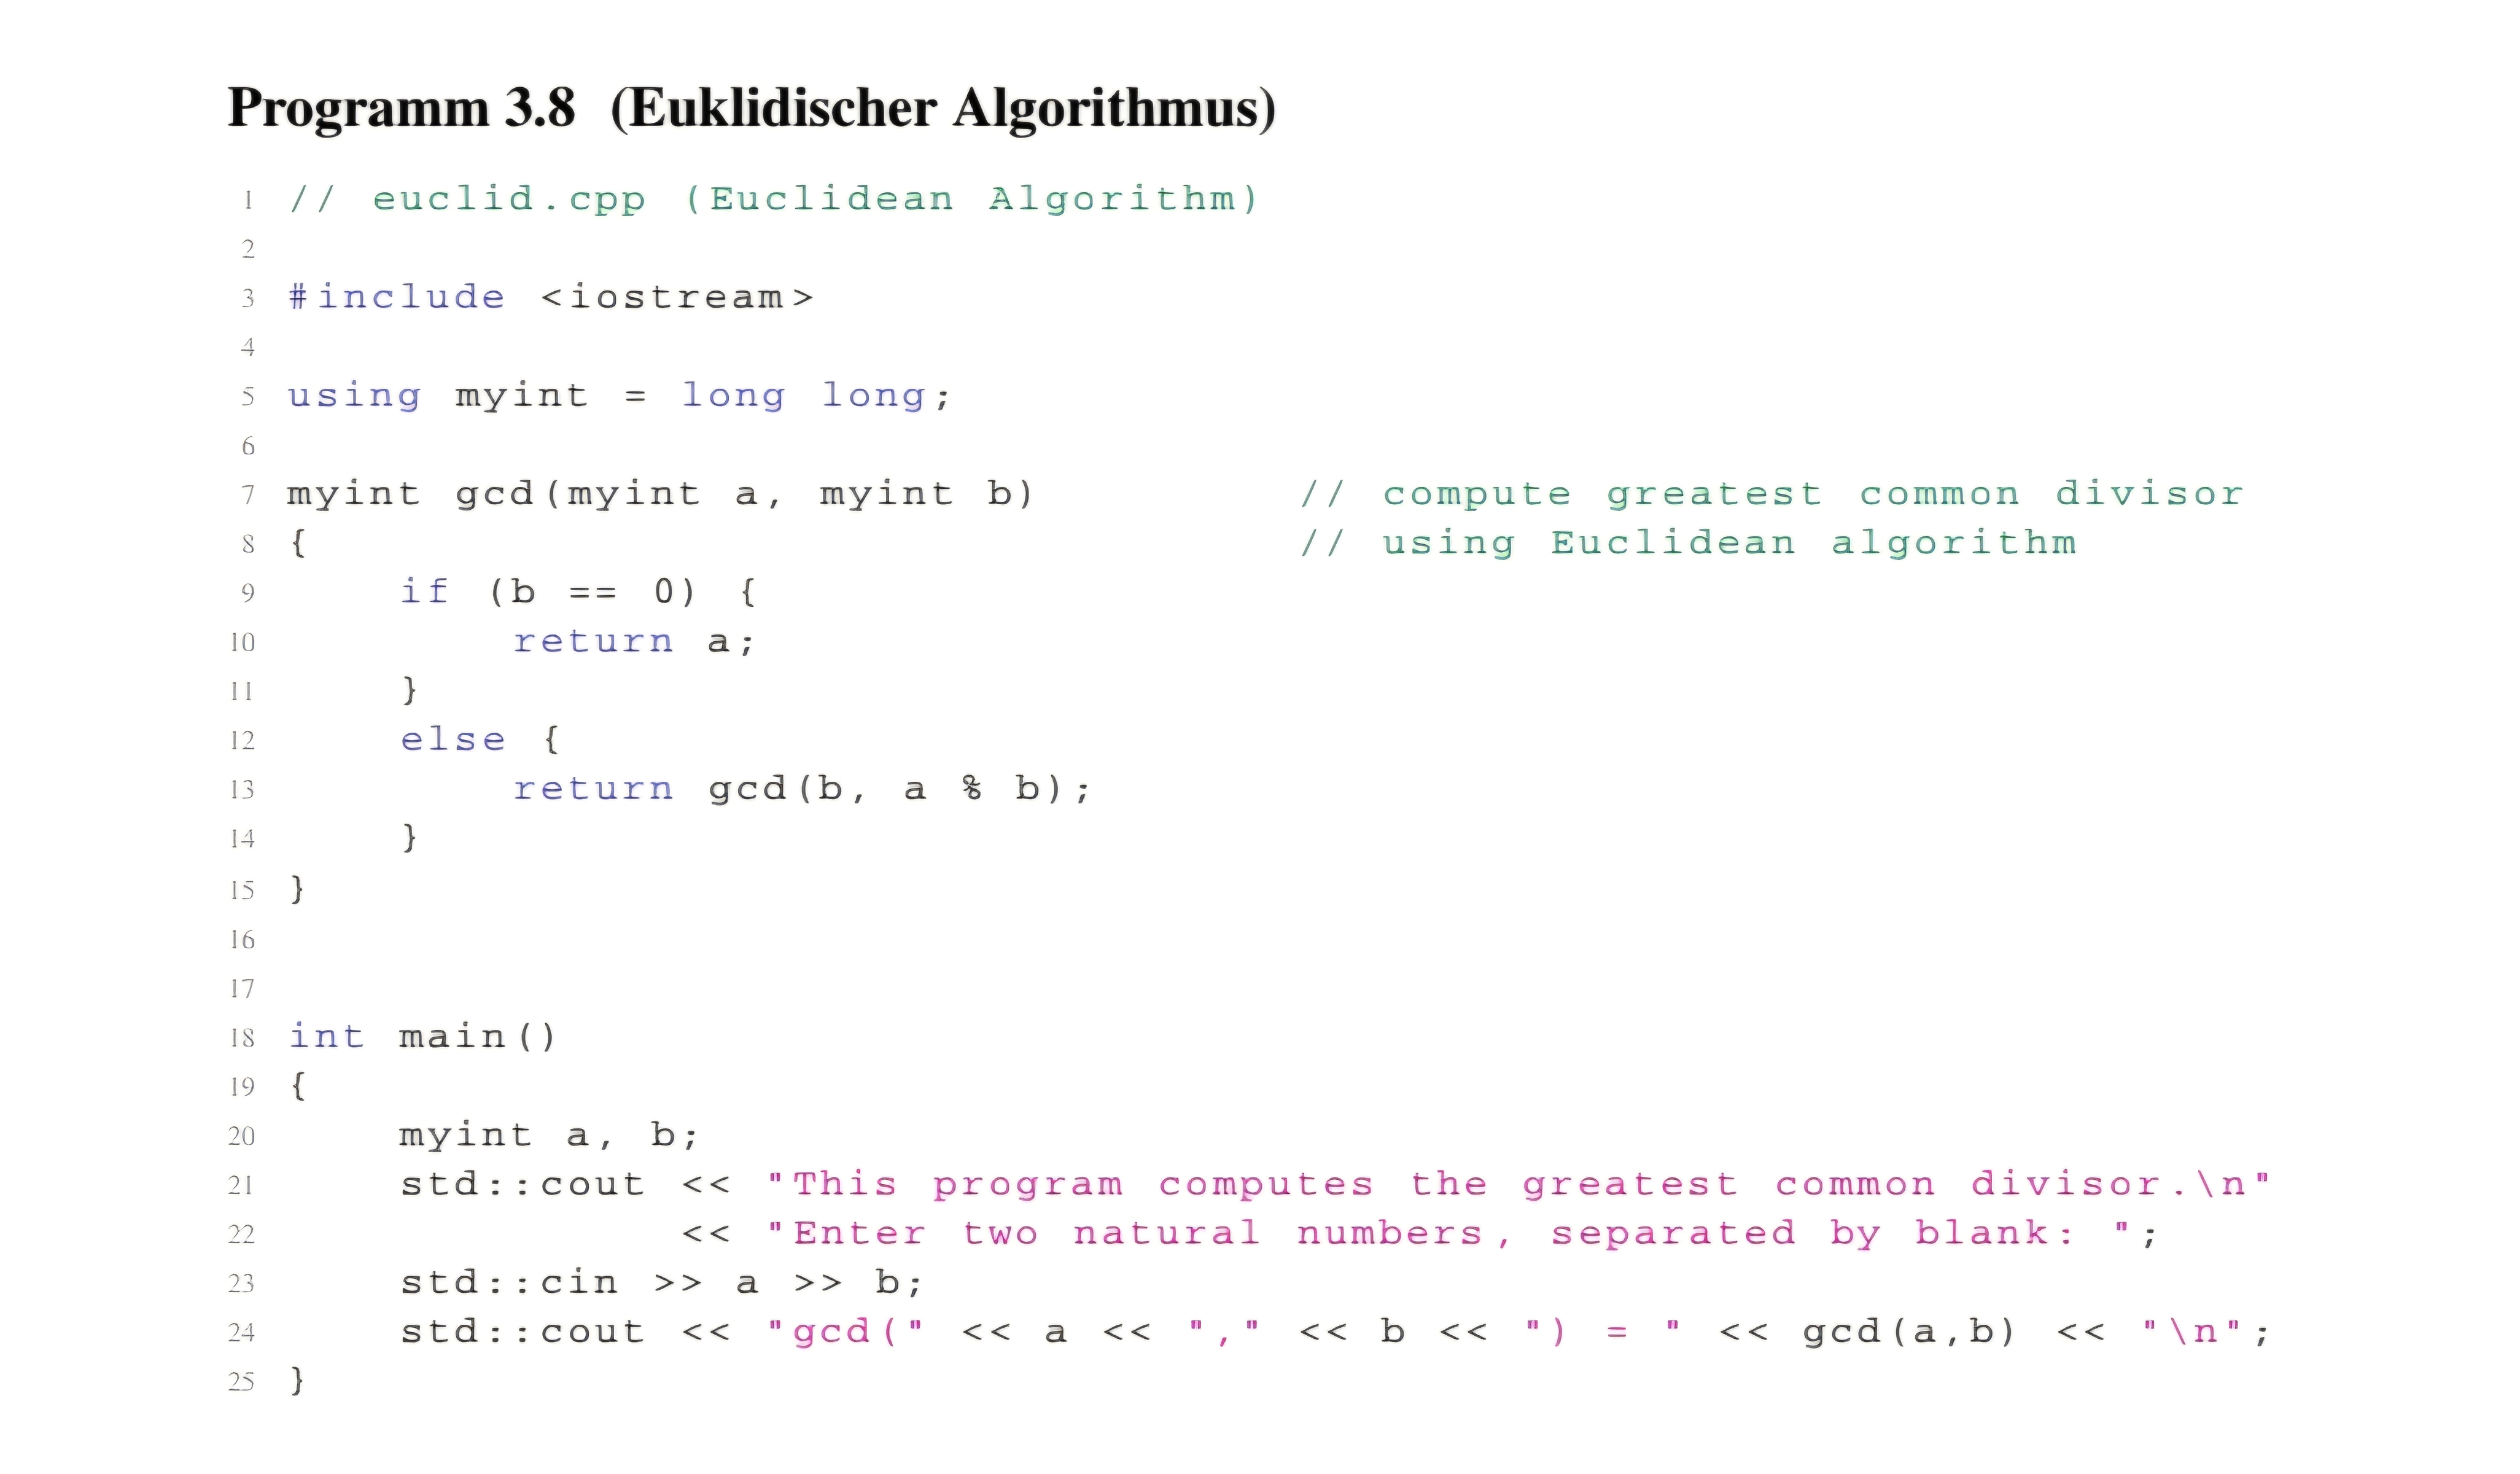
\includegraphics[width=1.1 \linewidth]{SmartSelect_20260410_212934_Samsung Notes.jpg}
    
    \label{fig:placeholder}
   
\end{figure}
    
\end{frame}

\begin{frame}
Formel für Laufzeit: 2 + \left\lfloor \log_2(\max\{a,1\}) \right\rfloor + \left\lfloor \log_2(\max\{b,1\}) \right\rfloor
    
\end{frame}

\begin{frame}{Definition 3.5: Fibonacci-Zahlen}

    Für eine genauere Analyse der Laufzeit des Euklidischen Algorithmus benötigen wird die Fibonacci Zahlen. Sie sind benannt nach Leonardo Fibonacci, welcher damit das Wachstum einer Kaninchenpopulation beschreib. Doch schon vor mehr als 400 Jahren vor Fibonacci waren diese Zahlen schon in Indien bekannt (ca. 1170-1240).
\end{frame}

\begin{frame}

 $F_i$ ist für $i= 0,1,2,3,4,...$ gegeben durch: 

\vspace{0.2cm}

$F_0:= 0$

$F_1:= 1$

$F_n+1:= F_n + F_n+1$

\vspace{0.2cm}

\noindent Die ersten Fibonacci Zahlen sehen wie folgt aus: $\{0,1,1,2,3,5,8,13,21,34,55\}\ $

\noindent D.h. jede Zahl ist die Summe der beiden vorherigen Zahlen.
    
\end{frame}

\begin{frame}{Lemma 3.6: Moivre-Binet Formel}

$\forall n \in \mathbf (N_0)$ ist: \[ F_n = \frac{1}{\sqrt{5}} \left( \left(\frac{1+\sqrt{5}}{2}\right)^n - \left(\frac{1-\sqrt{5}}{2}\right)^n \right) \] 


\noindent Eine explizite Formel zur Berechnung der n-ten Fibonacci Zahl $F_n$, ohne die vorherigen Zahlen berechnen zu müssen.

    
\end{frame}

\begin{frame}{Beweis Teil a:}
Eine Fibonacci Zahl ist die Summe ihrer beiden Vorgänger. Es gilt:

\vspace{0.2cm}
 $f(n+1)= f(n) + f(n-1)$.

 
\vspace{0.3cm}
\noindent Ansatz: $ f(n) = x^n $


\vspace{0.2cm}
$x^n+1 = x^n + x^{n-1}    \mid x^{n-1}$

$\Leftrightarrow x^2 = x+1 $

 $\Leftrightarrow x^2 -x- 1 = 0$ 
\vspace{0.15cm}


$ \Rightarrow x_1 = \frac{1 + \sqrt{5}}{2} ,  x_2= \frac{1 - \sqrt{5}}{2}$

    
\end{frame}

\begin{frame}

$OBdA: f(n)= Ax_1^n + Bx_2^n$

\vspace{0.2cm}
\noindent Um herauszufinden, was A und B sind, setzten wir n= 0 und n= 1 ein. 

\vspace{0.2cm}

Da  $f(0)= 0:  f(0)= A+B= 0  \Rightarrow B= -A$

Da $ f(1)= 1: f(1)= Ax_1+ Bx_2= 1 \Rightarrow Ax_1 - Ax_2= 1 \Leftrightarrow  A \frac{1 + \sqrt{5}}{2} -A \frac{1 - \sqrt{5}}{2}= 1 $

\vspace{0.15cm}

$\Rightarrow A= \frac{1}{\sqrt{5}} \ und  \ B= - \frac{1}{\sqrt{5}}$

\vspace{0.3cm}

\noindent Damit erhalten wir die gesuchte Formel: $f(n)= \frac{1}{\sqrt{5}} ((\frac{1 + \sqrt{5}}{2})^n - ( \frac{1 - \sqrt{5}}{2})^n)$.

    
\end{frame}

\begin{frame}{Teil b: Per Induktion}

I.A. $ F_0= f(n)= 
  \frac{1}{\sqrt{5}}((\frac{1 + \sqrt{5}}{2})^0 - ( \frac{1 - \sqrt{5}}{2})^0) = \frac{1}{\sqrt{5}} (1-1)= 0 $

\vspace{0.15cm}
    $F_1=  \frac{1}{\sqrt{5}} ((\frac{1 + \sqrt{5}}{2})^1 - ( \frac{1 - \sqrt{5}}{2})^1)= \frac{1}{\sqrt{5}} (\frac{2\sqrt{5}}{2}) = 1 $

\vspace{0.4cm}

\noindent I.V. von $n-1$ \ nach \ $ n-2$

$F_n= F_{n-1} + F_{n-2}$

\[
= \frac{1}{\sqrt{5}} \Bigg(
\left(\frac{1+\sqrt{5}}{2}\right)^{n-1}
+
\left(\frac{1+\sqrt{5}}{2}\right)^{n-2}
-
\left(\frac{1-\sqrt{5}}{2}\right)^{n-1}
-
\left(\frac{1-\sqrt{5}}{2}\right)^{n-2}
\Bigg)
\]
\[
= \frac{1}{\sqrt{5}} \Bigg(
\left(\frac{1+\sqrt{5}}{2}\right)^{n-2}
\left(\frac{1+\sqrt{5}}{2} + 1 \right)
-
\left(\frac{1-\sqrt{5}}{2}\right)^{n-2}
\left(\frac{1-\sqrt{5}}{2} + 1 \right)
\Bigg)
\]
\[
= \frac{1}{\sqrt{5}} \left(
\left(\frac{1+\sqrt{5}}{2}\right)^n
-
\left(\frac{1-\sqrt{5}}{2}\right)^n
\right)
\]
    
\end{frame}

\begin{frame}{Lemma 3.7}

Falls $a > b > 0$ und der Algorithmus 3.4 $k \geq 1$ Iterationen der while-Schleife durchläuft, so gilt: 


\vspace{0.25cm}
$a \geq F_{k+2} \ und \ b \geq F_{k+1}$

    
\end{frame}


\begin{frame}{Beispiel}

Ang. wir benötigen 3 Schritte, dann muss $b \geq 3= F_{3+1}$  sein und 

\noindent $a \geq 5= F_{3+2}$

\vspace{0.3cm}
$ggT(a,b)= ggT(5,3)= ggT(3,2)= ggT(2,0)= 2$ 
    
\end{frame}


\begin{frame}{Beweis von 3.7 per Induktion}

z.z.: $a \geq F_{k+2} \ und \ b \geq F_{k+1}$

\vspace{0.5cm}
 I.A.: k=1: $ b \geq F_{1+1}= 1$


  \indent $a \geq F_{1+2}= 2$

\noindent  Da $a > b > 0, und  \ b \in \mathbf{N}$, muss $b \geq 1$ sein und damit $a \geq 2$


\vspace{0.4cm}
\noindent I.S.: von (k-1) nach k.
\vspace{0.15cm}

$a \ mod \ b \geq F_{k}$, $ b \geq F_{k+1}$

\vspace{0.15cm}

Es gilt: $a= \lfloor \frac{a}{b} \rfloor \times b + (a \ mod \ b)$

\vspace{0.15cm}
Da $a > b: \lfloor \frac{a}{b} \rfloor > 1$ 

\vspace{0.3cm}
\noindent Damit folgt: $a= \lfloor \frac{a}{b} \rfloor \times b + (a \ mod \ b)
\geq b+ (a \ mod  \ b) \geq F_{k+1} + F_{k}= F_{k+2}$

\end{frame}


\begin{frame}{Satz von Lame 3.8}

Falls $a \geq b$ und $b > F_{k+1}$ für ein $k \in \mathbf{N}$, so durchläuft der Algorithmus 3.4 weniger als k Iterationen der while-Schleife.

    
\end{frame}

\begin{frame}{Beweis von 3.8}

Fall 1: Falls $ b= 0$: Algorithmus durchläuft gar keine Iterationen, d.h. $k=0$. Denn $ggT(a,b)= ggT(a,0)= a$.

\vspace{0.2cm}
\noindent Fall 2: Falls $a=b$: Algorithmus durchläuft nur eine Iteration. Denn: $ggT(a,b)= ggT(a,a)= ggT(a, a \ mod \ a)= ggT(a, 0) = a$.
    
\end{frame}

\begin{frame}{Korollar 3.9}

Falls $a \geq b > 1 $ , so durchläuft der Algorithmus 1.34 höchstens $\left\lceil \log_{\varphi} b \right\rceil$ Iterationen, wobei $\varphi = \frac{1 + \sqrt{5}}{2}$  (Goldener Schnitt).
Die Gesamtzeit des Algorithmus zur Berechnung von $ggT(a,b) ist = O ((log \ a)^3)$
    
\end{frame}

\begin{frame}{Beweis von 3.9 per Induktion}

Teil 1: 

\vspace{0.4cm}
 I.B.: $ F_n > \varphi ^{n-2}$


\vspace{0.3cm}
\indent I.A.: $ n=3: $

$F_3= 2 > \varphi ^ {3-2} = \varphi ^1$


\vspace{=0.3cm}


I.S.: $ F_n > \varphi ^{n-2}, F_{n-1} > \varphi ^ {n-3}$


\vspace{0.15cm}
Dann ist: $ F_{n+1}= F_n + F_ {n-1}$ 

$\Rightarrow F_{n+1} > \varphi ^{n-2} + \varphi ^ {n-3} = \varphi ^ {n-3} ( \varphi +1) = \varphi ^ {n-3} \times \varphi ^2$


\vspace{0.15cm}
 $Trick: 1+ \varphi = \varphi^2 $


 \vspace{0.15cm}
 Einsetzten: $F_{n+1} > \varphi ^{n-3} \times \varphi ^2$

    
\end{frame}


\begin{frame}

    Teil 2: 

\vspace{0.3cm}
 Setze $k= 1 + \left\lceil \log_{\varphi} b \right\rceil \geq 2$ 

 z.z. $b \leq  \varphi ^{k-1} < F_{k+1}$ 
 
\vspace{0.15cm}
 Gilt nach Satz von Lame.

\end{frame}

\begin{frame}

Teil 3: 
 \vspace{0.3cm}

Computer machte etwa $log b$ Iterationen. Da $ a \geq b : O(log \ a) $:

Division mit Schulmethode dauert bei n-stelligen Zahlen etwa $O(n^2)$.
\indent Also haben wir demnach: $O((log \ a)^2)$


\vspace{0.2cm}
$Anzahl \ Iterationen \times Anzahl \ Rechenschritte \ pro \ Iteration=$  

$O(log\ a) \times O((log \ a)^2) = O((log\ a)^3)$


    
\end{frame}

\begin{frame}{Literaturverzeichnis}

Hougardy, S. und  Vygen, J.: Algorithmische Mathematik 2., korrigierte und erweiterte Auflage. Berlin: Springer Spektrum, 2018.

    
\end{frame}

\end{document}
